\documentclass[conference]{IEEEtran}
\usepackage{cite}
\usepackage{amsmath,amssymb}
\usepackage{graphicx}
\usepackage{booktabs}
\usepackage{xcolor}
\usepackage[hidelinks]{hyperref}
\usepackage{orcidlink}
\usepackage{microtype}
\usepackage{fancyhdr}
\newcommand{\orcid}[1]{\,\orcidlink{#1}}
\newcommand{\correspondingemail}{\textcolor{repoLinkBlue}{\href{mailto:markus.baumann@campus.lmu.de}{markus.baumann@campus.lmu.de}}}
\fancypagestyle{firstpagecorresp}{
    \fancyhf{}
    \fancyfoot[L]{\footnotesize Corresponding author: \correspondingemail}
    \fancyfoot[C]{\thepage}
    \renewcommand{\headrulewidth}{0pt}
    \renewcommand{\footrulewidth}{0pt}
}
\setlength{\textfloatsep}{4pt plus 1pt minus 2pt}
\setlength{\floatsep}{4pt plus 1pt minus 1pt}
\setlength{\intextsep}{4pt plus 1pt minus 1pt}
% --- float placement: allow full-width (double) floats to fill more of a page ---
\renewcommand{\dbltopfraction}{0.92}
\renewcommand{\dblfloatpagefraction}{0.80}
\renewcommand{\topfraction}{0.92}
\renewcommand{\bottomfraction}{0.70}
\renewcommand{\textfraction}{0.06}
\renewcommand{\floatpagefraction}{0.80}
\setcounter{dbltopnumber}{2}
\setcounter{topnumber}{3}
\renewcommand{\arraystretch}{1.04}
\newcommand{\MC}{\mathrm{MC}}
\newcommand{\NMSE}{\mathrm{NMSE}}
\definecolor{repoLinkBlue}{RGB}{0,92,184}
% Auto-generated by scripts/analyze_phase_map_generalization.py
\newcommand{\PhasePrimaryBand}{$B_{20,0.7}$}
\newcommand{\PhaseBTwentyQSeventySize}{4}
\newcommand{\PhaseBTwentyQSeventyComponents}{1}
\newcommand{\PhaseBTwentyQSeventyLargest}{4}
\newcommand{\PhaseBTwentyQSixtySize}{14}
\newcommand{\PhaseBThirtyQSeventySize}{46}
\newcommand{\PhaseRepresentativeBetaPi}{0.04}
\newcommand{\PhaseRepresentativeLambdaPi}{0.12}
\newcommand{\PhaseRepresentativeGamma}{0.12}
\newcommand{\PhaseLotoMeanRank}{0.240}
\newcommand{\PhaseLotoCILow}{0.215}
\newcommand{\PhaseLotoCIHigh}{0.265}
\newcommand{\PhaseLosoMeanRank}{0.180}
\newcommand{\PhaseLosoCILow}{0.154}
\newcommand{\PhaseLosoCIHigh}{0.209}
\newcommand{\PhaseMCSpearman}{-0.85}
\newcommand{\PhaseIPCmemSpearman}{-0.84}
\newcommand{\PhaseIPCtotSpearman}{-0.90}
\newcommand{\PhaseIPCnonlinSpearman}{-0.80}
\newcommand{\PhaseVfeatSpearman}{0.16}
\newcommand{\PhaseReffSpearman}{0.15}
\newcommand{\PhaseAblationBaseBandSize}{4}
\newcommand{\PhaseGammaZeroRetention}{0.00}
\newcommand{\PhaseNoMixerRetention}{0.00}
\newcommand{\PhaseDephaseRetention}{0.00}
\newcommand{\PhaseAblationRows}{base AD+RxZZ & 4 & 1.00 & 0.256\\
$\gamma=0$ & 0 & 0.00 & 0.465\\
dephasing & 0 & 0.00 & 0.442\\
depolarizing & 0 & 0.00 & 0.526\\
no mixer & 0 & 0.00 & 0.403\\
Rx only & 0 & 0.00 & 0.521\\
ZZ only & 0 & 0.00 & 0.503\\}

\begin{document}
\title{Where a Quantum Reservoir Works: A Transferable Operating Band}
\author{%
\IEEEauthorblockN{%
Markus Baumann\IEEEauthorrefmark{1}\orcid{0009-0007-3575-1006},
Itamar Fink\IEEEauthorrefmark{1}\orcid{0009-0000-2262-4445},
Johannes Wittmann\IEEEauthorrefmark{1}\orcid{0009-0009-9240-7257},
and Jonas Stein\IEEEauthorrefmark{1}\orcid{0000-0001-5727-9151}}
\IEEEauthorblockA{\IEEEauthorrefmark{1}\textit{QAR-Lab, Department of Computer Science, LMU Munich, Munich, Germany}}
}
\maketitle
\thispagestyle{firstpagecorresp}

\begin{abstract}
In quantum reservoir computing, a fixed quantum system transforms an input signal and learning reduces to training a simple linear readout on its measured outputs. Because the quantum dynamics are never optimized, the method suits today's hardware. This raises an obvious question: where in its control space does a fixed quantum system become good at learning? We answer it for a dissipative reservoir by mapping performance over its three central physical control parameters: the input-rotation strength $\beta$, the nearest-neighbor $ZZ$ coupling $\lambda$, and the amplitude-damping rate $\gamma$. Good performance does not scatter across these settings; it concentrates in a well-defined operating region. This region transfers: identified on one set of tasks, it reliably locates good settings for new tasks and new reservoir initializations, and the same memory-defined regime persists when the architecture changes. We confirm it is real by showing it collapses when any mechanism that creates it is removed, and that it can be located cheaply and in advance using a simple memory diagnostic. Reservoir tuning thus becomes a search for a transferable, memory-preserving regime rather than a hunt for one benchmark-specific optimum.
\end{abstract}

\begin{IEEEkeywords}
quantum machine learning, reservoir computing, quantum computing, dissipative systems, memory capacity
\end{IEEEkeywords}

\begin{figure*}[t!]
\centering
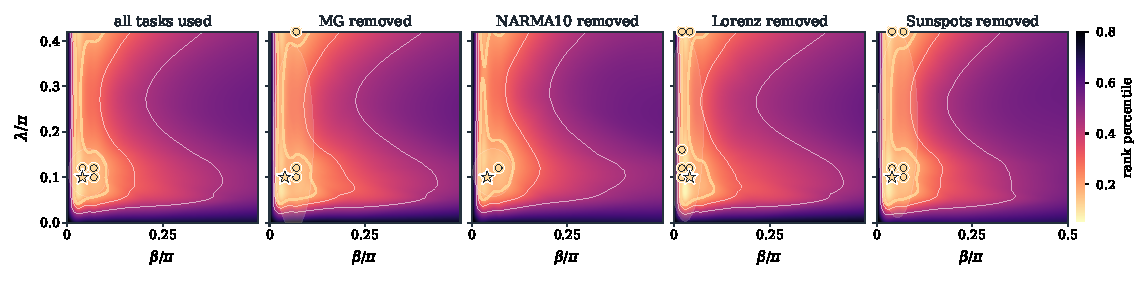
\includegraphics[width=\textwidth]{gfx/fig1_short_phase_maps.pdf}
\caption{\footnotesize Fig. 1. The good operating region is essentially the same whichever task we score. Each panel maps validation rank over input drive $\beta$ and coupling $\lambda$ at fixed damping $\gamma=0.12$, one slice of the range over which the band persists (Fig.~\ref{fig:gamma-slices} shows the band across $\gamma=0.12$--$0.30$). Brighter means better rank. Panel~(a) uses all four tasks; (b)--(e) each drops one. Gold circles mark the top validation quintile across tasks and seeds; the star is the band’s medoid (center). The basin and circles barely move when a task is dropped, so the band is not an artifact of any single task.}
\label{fig:phase}
\end{figure*}

\section{Introduction}
Reservoir computing rests on an economical idea: a fixed dynamical system, left untrained, transforms an input signal into a high-dimensional trace of its recent history, and learning reduces to fitting a single linear readout on top of that trace \cite{maass2002,jaeger2004,lukosevicius2009,tanaka2019}. The dynamics are never optimized, only observed. This economy is precisely what makes the approach appealing for near-term quantum hardware: native quantum evolution can serve as the reservoir and only the classical readout must be trained \cite{fujii2017,ghosh2019,chen2020,mujal2021}. Yet the same economy relocates the burden of the method onto the fixed dynamics, and so onto a question that is easy to state and surprisingly hard to answer: what makes those dynamics useful?

Recent QRC work now spans noisy gate-model devices, continuous-variable and oscillator reservoirs, weak-measurement protocols, photonic reservoirs, noise-engineered reservoirs, and experimental optical memory control \cite{nokkala2021,govia2021,mujal2023,kubota2023,garciabeni2023,paparelle2026}. Classical reservoir theory has long since refused the obvious answer. Usefulness is not maximal expressivity. A reservoir works by holding a balance: retaining recent input, forgetting old input in a controlled way, and exposing nonlinear functions of that history to the readout \cite{dambre2012,tanaka2019}. A quantum reservoir inherits this lesson but complicates it, because these ingredients are no longer free dials. They are consequences of distinct physical resources: how strongly the input perturbs the carried state, how coherently the system mixes that state across its parts, and how it is allowed to dissipate \cite{chen2020,martinezpena2023,sannia2024}.

We take this as an organizing principle rather than a caveat. For a stateful dissipative gate-model reservoir, we treat the space of these three resources as the proper setting in which to ask when the reservoir works, and we map it. The picture that emerges is not a single tuned operating point but a connected region---gentle input, nonmaximal coupling, controlled damping---in which good performance concentrates and from which it does not stray arbitrarily across tasks. The contribution of this paper is that region itself: its existence, its transfer across tasks and reservoir initializations, the mechanisms that sustain it, and a memory-based diagnostic that locates it before any task-specific search.

\section{Protocol}
\subsection{Reservoir}
The reservoir processes a scalar time series without resetting its density matrix, so the carried state stores recent history. We write $\rho_{t,\ell}$ for the quantum state after input time $t$ and layer $\ell$; $L$ is the final layer, so $\rho_{t-1,L}$ is the state carried over from the previous time step. At step $t$, the scalar input value $u_t$ perturbs this carried state through the same $Y$ rotation on every qubit,
\begin{equation}
\rho_{t,0}
=U_{\mathrm{in}}(u_t)\rho_{t-1,L}U_{\mathrm{in}}^\dagger(u_t),
\qquad
U_{\mathrm{in}}(u_t)=\bigotimes_i R_y(\beta u_t).
\end{equation}
Here $R_y(\cdot)$ is a single-qubit rotation, $\bigotimes_i$ means that the rotation is applied to all qubits, and $^\dagger$ denotes the inverse conjugate transpose. The input strength $\beta$ controls how strongly each step writes into the carried state.

The perturbed state then passes through identical layers: a frozen local mixer $U_{\rm mix}$, a ring $ZZ$ coupling unitary $U_\lambda$, and a dissipative channel $\mathcal{D}_\gamma$ applied independently to all $n$ qubits,
\begin{equation}
\begin{aligned}
\rho_{t,\ell}
&=\mathcal{D}_{\gamma}^{\otimes n}\!\left[
U_\lambda U_{\rm mix}\rho_{t,\ell-1}
U_{\rm mix}^\dagger U_\lambda^\dagger\right],\\
U_\lambda
&=\prod_{(i,j)\in E_{\rm ring}}e^{-i\lambda Z_iZ_j}.
\end{aligned}
\end{equation}
In this expression, $E_{\rm ring}$ is the set of nearest-neighbor edges on the qubit ring, $Z_i$ is the Pauli-$Z$ operator on qubit $i$, $\lambda$ sets the coupling strength, and $\gamma$ sets the damping rate. We vary only $\theta=(\beta,\lambda,\gamma)$, where $\beta$ and $\lambda$ are angles in radians and $\gamma\in[0,1]$ is the amplitude-damping probability; all other gates are frozen and only a linear readout is trained. Each control corresponds to one ingredient required by reservoir theory: $\beta$ governs how new information competes with old memory, $\lambda$ generates nonlinear mixing of past inputs, and $\gamma$ provides the controlled forgetting on which fading memory depends.

This is a minimal testbed, not an optimized model. Four qubits and two layers keep the phase grid searchable, the ring coupling still gives recurrent many-body mixing, and the modest $Z+ZZ$ readout observes local and nearest-neighbor correlations rather than the full density matrix.

\subsection{Configuration}
Unless stated otherwise, the reservoir has four qubits and two layers with ring coupling, uniform input injection, and amplitude damping; the readout takes single-qubit $Z$ and ring-pair $ZZ$ expectations, and training is ridge regression on these features alone. We sweep $\beta/\pi\in\{0,0.02,0.04,0.07,0.10,0.22,0.50\}$, $\lambda/\pi\in\{0,0.05,0.10,0.12,0.16,0.28,0.42\}$, and $\gamma\in\{0,0.01,0.05,0.12,0.22,0.30\}$, and select every hyperparameter including the ridge penalty on validation only—holdout is never used to define the operating region. Crossing the four benchmark tasks with twenty frozen-reservoir seeds yields a balanced panel of $80$ task-seed replicates per grid coordinate. This full factorial is fixed in advance, not chosen after seeing results, so that the leave-one-task and leave-one-seed transfer checks below all rest on the same uniform design.

\subsection{Tasks, Metric, and Splits}
We use four scalar one-step-ahead prediction tasks chosen to span distinct demands: Mackey–Glass and the Lorenz $x$-coordinate for smooth chaos \cite{mackey1977,lorenz1963}, NARMA for nonlinear memory \cite{narendra1990}, and annual sunspot counts for irregular real-world data. Inputs are scaled to $[-1,1]$ and targets standardized. We use splits $(w,\mathrm{tr},\mathrm{va},\mathrm{te})=(300,1600,400,400)$ for Mackey--Glass, Lorenz, and NARMA, and $(20,150,50,60)$ for sunspots. We score with normalized mean-squared error (NMSE), the mean squared error divided by target variance, so predicting the mean alone scores $1$ and lower is better; it is computed separately on validation and holdout. The ridge penalty is selected by validation NMSE alone from $\{10^{-8},10^{-7},\ldots,10^3\}$.

\subsection{Operating Band}
To locate the useful region we rank performance within each task $j$ and seed $s$. A setting $\theta\in\Theta_{\rm grid}$ receives validation percentile rank $r_{j,s}(\theta)$, with lower rank better. The operating band contains settings that land in the top fraction $p$ for at least a fraction $q$ of task-seed pairs,
\begin{equation}
B_{p,q}=\{\theta:\Pr_{j,s}[r_{j,s}(\theta)\le p]\ge q\}.
\end{equation}
This frequency-level criterion is a selection-stability test in the spirit of stability selection~\cite{meinshausen2010}: instead of asking which single coordinate wins, it keeps the settings chosen often across replicates and so treats the band as a search prior over settings that reliably work. We report the strict band $B_{20,0.7}$---top-quintile rank on at least a $70\%$ supermajority of the task-seed replicates. These thresholds are conventional rather than tuned, and the band does not depend on their exact values: relaxing either one enlarges the same region smoothly and connectedly rather than fragmenting it, from \PhaseBTwentyQSeventySize{} grid coordinates at $B_{20,0.7}$ to \PhaseBTwentyQSixtySize{} at $B_{20,0.6}$ and \PhaseBThirtyQSeventySize{} at $B_{30,0.7}$, the signature of a single operating regime. In leave-one-task or leave-one-seed tests, the band is built from the remaining replicates and scored on the withheld replicate. In the holdout audit, the validation-defined band is frozen first and evaluated once on holdout ranks and NMSE. Confidence intervals are nonparametric bootstrap percentile intervals for the mean with 50,000 resamples and a fixed seed. Because ranks are formed within each task-seed replicate before aggregation, no large-error task or difficult seed can dominate the band.

\section{Results}
Across the control space, low validation rank does not spread arbitrarily; it gathers into a compact, connected region rather than a scatter of isolated optima (Fig.~\ref{fig:phase}). The damping coordinate is selected by validation, not fixed by hand: the near-zero $\gamma=0.01$ slice is a weak contrast, while the strict $B_{20,0.7}$ core appears for $\gamma=0.12$--$0.30$ with medoid $\gamma=\PhaseRepresentativeGamma$ (Fig.~\ref{fig:gamma-slices}). We use $\gamma=0.12$ in Fig.~\ref{fig:phase} because it is the first populated band slice, not because it was chosen as a magic operating point. To establish that the band is a genuine transferable prior rather than a joint fit to these four tasks, we test whether it survives removal of the information it was built from. It does: when one task is withheld, the band built from the rest scores mean held-out rank \PhaseLotoMeanRank{} with CI $[\PhaseLotoCILow,\PhaseLotoCIHigh]$; when one seed is withheld, the corresponding mean rank is \PhaseLosoMeanRank{} with CI $[\PhaseLosoCILow,\PhaseLosoCIHigh]$. Since rank is normalized so that $0.5$ is chance, both values sit deep in the top quartile, and the band therefore generalizes across task identity and reservoir initialization alike.

\begin{figure}[t!]
\centering
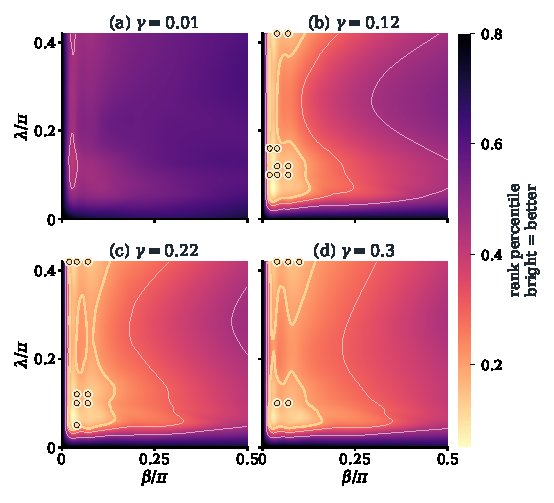
\includegraphics[width=\columnwidth]{gfx/fig4_gamma_slices_compact.pdf}
\caption{Damping is selected by the data, not set by hand. Each panel shows validation rank over $(\beta,\lambda)$ at one damping rate $\gamma$ (brighter $=$ better); gold circles are the band coordinates in that slice. Almost nothing qualifies at near-zero damping ($\gamma=0.01$); the band appears and strengthens once damping is present ($\gamma=0.12$--$0.30$), so controlled forgetting is necessary for the regime.}
\label{fig:gamma-slices}
\end{figure}

The frozen band also holds on data it never touched: evaluated once on the chronological holdout, it stays in the top quartile on every task (Table~\ref{tab:holdout}). The regime is, moreover, a property of the dynamics rather than of one architecture. A four-qubit, three-layer variant again forms a band whose held-out performance matches the base model ($0.154$ vs.\ $0.153$), even though its exact coordinates shift (Jaccard overlap $0.04$). This is exactly what we expect if what transfers is a memory-defined regime rather than a fixed operating point, and it is why a task-free diagnostic, not a memorized location, is the right way to find it.

Mechanism ablations confirm that the regime is causal rather than incidental. Removing damping, removing the recurrent mixer, replacing amplitude damping with dephasing or depolarizing noise, or restricting the readout to $Z$-only or $ZZ$-only features each erases the band entirely (retention $0.00$ in every case; Table~\ref{tab:ablation}), and the resulting rank loss concentrates exactly where the base band sat (Fig.~\ref{fig:evidence}). The band thus requires the full combination of write-without-overwrite input, nonlinear mixing, and usable memory; remove any one and the region does not weaken, it disappears. Finally, the band can be located before any task is run: memory capacity correlates strongly with validation rank, $\rho_s=\PhaseMCSpearman{}$, as do information-processing capacities~\cite{dambre2012}, whereas raw feature diversity does not (Fig.~\ref{fig:diagnostics}).

\begin{figure}[t!]
\centering
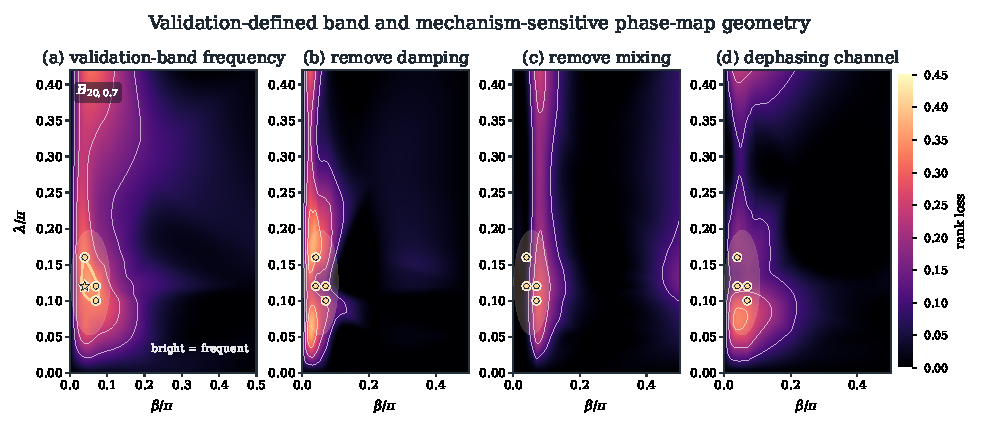
\includegraphics[width=\columnwidth]{gfx/fig2_short_evidence.pdf}
\caption{The band is held in place by specific physical mechanisms. (a)~How often each coordinate is selected into the band $B_{20,0.7}$ (brighter $=$ more frequent); gold circles are the band. (b)--(d)~Increase in validation rank when damping is removed, the recurrent mixer is removed, or amplitude damping is replaced by dephasing (darker $=$ larger loss). The loss lands exactly on the gold band in every case, so the useful region depends on these mechanisms rather than appearing by chance.}
\label{fig:evidence}
\end{figure}

\begin{figure*}[t!]
\centering

\includegraphics[width=\textwidth]{gfx/fig3_memory_capacity_screens.pdf}
\caption{Memory alone locates the band, before any task is run. (a)~Task-free memory map $\log(1+\mathrm{MC})$ on the same $\gamma=0.12$ slice as Fig.~\ref{fig:phase}; the gold band points lie inside the memory-rich region, so the band is visible from the reservoir's dynamics alone. (b)~Across all settings and seeds, higher memory predicts better (lower) validation rank (Spearman $\rho_s=-0.88$). (c)~Keeping only the top-ranked fraction of settings according to a cheap diagnostic, the fraction of genuinely good reservoirs retained: memory ($\mathrm{MC}$) and information-processing capacity ($\mathrm{IPC}$) recover them far faster than random selection, while raw feature diversity ($V_{\mathrm{feat}}$) barely beats chance.}
\label{fig:diagnostics}
\end{figure*}

\begin{table}[t]
\centering
\scriptsize
\caption{Holdout performance after validation-only band selection. Means are over twenty seeds per task; ``All'' averages the 80 task-seed rows.}
\label{tab:holdout}
\setlength{\tabcolsep}{3.2pt}
\begin{tabular}{@{}lccc@{}}
\toprule
Task & Band NMSE & Medoid NMSE & Band rank\\
\midrule
\PhaseHoldoutRows
\bottomrule
\end{tabular}
\end{table}

\begin{table}[t]
\centering
\scriptsize
\caption{Mechanism ablations. Each row alters one ingredient and re-selects the band under the same criterion. Only the full model sustains a band; every alternative collapses to no band points and chance-level rank (0.5) at the original coordinates.}
\label{tab:ablation}
\setlength{\tabcolsep}{3.2pt}
\begin{tabular}{@{}lccc@{}}
\toprule
Mechanism & Band pts. & Retention & Rank at base band\\
\midrule
\PhaseAblationRows
\bottomrule
\end{tabular}
\end{table}

\section{Discussion and Conclusion}
For this reservoir family, useful learning is organized by a transferable operating regime rather than by task-specific tuning: four tasks spanning smooth chaos, nonlinear memory, and irregular real-world data obey the same region, and that region holds when any one task or seed is withheld. The region is picked out not by Hilbert-space size or raw feature diversity but by memory, so that drive, coupling, and dissipation keep memory and nonlinearity in the balance classical reservoir theory identified~\cite{dambre2012,tanaka2019}. This is also why the ablations bite---strip out damping or mixing and the regime does not merely weaken, it disappears---and why a task-free memory diagnostic can locate the region before any task is run. The usefulness of a dissipative quantum reservoir is thus not a property of its size but of where it is operated. The scope is deliberately narrow: all results are simulated on one architecture family with measurement treated as free, so finite-shot noise, calibration drift, device noise, and readout cost lie outside the present claim~\cite{mujal2023,ahmed2025}. We claim neither quantum advantage nor hardware efficiency---only that the operating regime is the right object to study, that it transfers, and that memory is how to find it.

\section*{Reproducibility Appendix}
\subsection{Package}
The \href{https://github.com/eybmits/qrc_operating_band}{\textcolor{repoLinkBlue}{project repository}} contains the code, checked-in CSV/JSON results, and final figures used in this paper.

\subsection{Frozen reservoir}
The simulator evolves the full density matrix exactly, with no finite-shot sampling. It starts from $\rho_0=|0\cdots0\rangle\langle0\cdots0|$ and carries state between time steps without reset. For each seed, \texttt{default\_rng(s)} draws one fixed mixer $U_{\rm mix}=\bigotimes_iR_x(\theta_i)$, $\theta_i\sim U[0,2\pi)$, reused at every step and layer. Each layer applies $U_\lambda U_{\rm mix}$ on ring edges, then local amplitude damping. The readout is ridge regression on exact $Z_i$ and ring-pair $Z_iZ_j$ expectations with an unpenalized intercept.

\subsection{Selection and diagnostics}
The full control grid is $\mathcal{B}=\{0,0.02,0.04,0.07,0.10,0.22,0.50\}$, $\mathcal{L}=\{0,0.05,0.10,0.12,0.16,0.28,0.42\}$, and $\mathcal{G}=\{0,0.01,0.05,0.12,0.22,0.30\}$. The fixed task splits are $(w,\mathrm{tr},\mathrm{va},\mathrm{te})=(300,1600,400,400)$ for Mackey--Glass, Lorenz, and NARMA, and $(20,150,50,60)$ for sunspots. Ridge penalties $\{10^{-8},\ldots,10^3\}$ are chosen by validation NMSE only; holdout data are used only after the band is fixed. MC/IPC diagnostics use an independent $U[-1,1]$ drive of length 900, washout 150, ridge $\alpha=10^{-8}$, and a 70/30 chronological split. MC sums held-out positive $R^2$ over delays 1--10. IPC adds linear delays 1--20, quadratic Legendre delays 1--10, and ten cross-delay products, clipping negative $R^2$ to zero. CIs are nonparametric bootstrap percentile intervals with 50,000 resamples and a fixed seed.

\enlargethispage{2\baselineskip}
{\footnotesize
\begin{thebibliography}{99}
\setlength{\itemsep}{-0.4ex}
\setlength{\parskip}{0pt}
\bibitem{maass2002} W. Maass, T. Natschl\"{a}ger, and H. Markram, ``Real-time computing without stable states: A new framework for neural computation based on perturbations,'' \emph{Neural Computation}, vol. 14, no. 11, pp. 2531--2560, 2002.
\bibitem{jaeger2004} H. Jaeger and H. Haas, ``Harnessing nonlinearity: Predicting chaotic systems and saving energy in wireless communication,'' \emph{Science}, vol. 304, no. 5667, pp. 78--80, 2004.
\bibitem{lukosevicius2009} M. Luko\\v{s}evi\\v{c}ius and H. Jaeger, ``Reservoir computing approaches to recurrent neural network training,'' \emph{Computer Science Review}, vol. 3, no. 3, pp. 127--149, 2009.
\bibitem{tanaka2019} G. Tanaka \emph{et al.}, ``Recent advances in physical reservoir computing: A review,'' \emph{Neural Networks}, vol. 115, pp. 100--123, 2019.
\bibitem{fujii2017} K. Fujii and K. Nakajima, ``Harnessing disordered-ensemble quantum dynamics for machine learning,'' \emph{Physical Review Applied}, vol. 8, p. 024030, 2017.
\bibitem{ghosh2019} S. Ghosh, A. Opala, M. Matuszewski, T. Paterek, and T. C. H. Liew, ``Quantum reservoir processing,'' \emph{npj Quantum Information}, vol. 5, p. 35, 2019.
\bibitem{chen2020} J. Chen, H. I. Nurdin, and N. Yamamoto, ``Temporal information processing on noisy quantum computers,'' \emph{Physical Review Applied}, vol. 14, p. 024065, 2020.
\bibitem{mujal2021} P. Mujal \emph{et al.}, ``Opportunities in quantum reservoir computing and extreme learning machines,'' \emph{Advanced Quantum Technologies}, vol. 4, p. 2100027, 2021.
\bibitem{nokkala2021} J. Nokkala \emph{et al.}, ``Gaussian states of continuous-variable quantum systems provide universal and versatile reservoir computing,'' \emph{Communications Physics}, vol. 4, p. 53, 2021.
\bibitem{govia2021} L. C. G. Govia \emph{et al.}, ``Quantum reservoir computing with a single nonlinear oscillator,'' \emph{Physical Review Research}, vol. 3, p. 013077, 2021.
\bibitem{mujal2023} P. Mujal, R. Mart\'{i}nez-Pe\~{n}a, G. L. Giorgi, M. C. Soriano, and R. Zambrini, ``Time-series quantum reservoir computing with weak and projective measurements,'' \emph{npj Quantum Information}, vol. 9, p. 16, 2023.
\bibitem{kubota2023} T. Kubota \emph{et al.}, ``Temporal information processing induced by quantum noise,'' \emph{Physical Review Research}, vol. 5, p. 023057, 2023.
\bibitem{garciabeni2023} J. Garc{\'i}a-Beni, G. L. Giorgi, M. C. Soriano, and R. Zambrini, ``Scalable photonic platform for real-time quantum reservoir computing,'' \emph{Physical Review Applied}, vol. 20, p. 014051, 2023.
\bibitem{paparelle2026} I. Paparelle \emph{et al.}, ``Experimental memory control in continuous-variable optical quantum reservoir computing,'' \emph{Nature Photonics}, vol. 20, pp. 413--420, 2026.
\bibitem{dambre2012} J. Dambre, D. Verstraeten, B. Schrauwen, and S. Massar, ``Information processing capacity of dynamical systems,'' \emph{Scientific Reports}, vol. 2, p. 514, 2012.
\bibitem{meinshausen2010} N. Meinshausen and P. B\"{u}hlmann, ``Stability selection,'' \emph{Journal of the Royal Statistical Society: Series B (Statistical Methodology)}, vol. 72, no. 4, pp. 417--473, 2010.
\bibitem{martinezpena2023} R. Mart{\'i}nez-Pe\~{n}a and J.-P. Ortega, ``Quantum reservoir computing in finite dimensions,'' \emph{Physical Review E}, vol. 107, p. 035306, 2023.
\bibitem{sannia2024} A. Sannia, R. Mart{\'i}nez-Pe\~{n}a, M. C. Soriano, G. L. Giorgi, and R. Zambrini, ``Dissipation as a resource for quantum reservoir computing,'' \emph{Quantum}, vol. 8, p. 1291, 2024.
\bibitem{mackey1977} M. C. Mackey and L. Glass, ``Oscillation and chaos in physiological control systems,'' \emph{Science}, vol. 197, no. 4300, pp. 287--289, 1977.
\bibitem{lorenz1963} E. N. Lorenz, ``Deterministic nonperiodic flow,'' \emph{Journal of the Atmospheric Sciences}, vol. 20, no. 2, pp. 130--141, 1963.
\bibitem{narendra1990} K. S. Narendra and K. Parthasarathy, ``Identification and control of dynamical systems using neural networks,'' \emph{IEEE Transactions on Neural Networks}, vol. 1, no. 1, pp. 4--27, 1990.
\bibitem{ahmed2025} O. Ahmed, F. Tennie, and L. Magri, ``Optimal training of finitely sampled quantum reservoir computers for forecasting of chaotic dynamics,'' \emph{Quantum Machine Intelligence}, vol. 7, p. 31, 2025.
\end{thebibliography}
}
\end{document}
